% answers.tex —— 1980 年·全国卷（文科） · 参考答案与详细解析片段
% 由 tools/generate_projects.py 依来源总账自 1980/1980_数学真题_文_试题.md + 1980/1980_数学真题_文_解析正文.md + 1980/1980_数学真题_文_答案要点.md 生成，勿手改（改源 MD 后重跑）


\begin{gknotice}
\textbf{解析归属}：本卷仅题面、无答案页。下列解析由本库逐题独立推导并复算，不声称代表官方发布的标准答案。

\textbf{编注}：第 5 题被开方数经页面图像放大确认为\textbf{整个分子}（含方括号一项），故方括号中两项也必须计入被开方式；若漏读为只开 $\cos\frac{\pi}{4}\sin\left(\frac{3\pi}{4}-\theta\right)$，被开方式在题设区间内为负，根式无实义。第 7 题“$AE$ 与底面的对角线 $B'D'$ 垂直于 $E$”按“$AE\perp B'D'$、垂足为 $E$”理解。
\end{gknotice}

\begin{answer}
\gksolhead{1}{}

\textbf{题目}：

化简：$\dfrac{1-3\mathrm i}{3-2\mathrm i}$。

\Needspace{4\baselineskip}
\textbf{解析}

\Needspace{5\baselineskip}
分子分母同乘分母的共轭复数 $3+2\mathrm i$：
\nopagebreak[4]
\[
\frac{1-3\mathrm i}{3-2\mathrm i}
=\frac{(1-3\mathrm i)(3+2\mathrm i)}{(3-2\mathrm i)(3+2\mathrm i)}
=\frac{3+2\mathrm i-9\mathrm i-6\mathrm i^2}{3^2+2^2}
=\frac{9-7\mathrm i}{13}
=\frac{9}{13}-\frac{7}{13}\mathrm i.
\]

复算：$\left(\dfrac{9}{13}-\dfrac{7}{13}\mathrm i\right)(3-2\mathrm i)=\dfrac{27-18\mathrm i-21\mathrm i+14\mathrm i^2}{13}=\dfrac{13-39\mathrm i}{13}=1-3\mathrm i$，与原分子一致。

\gkanswer{答案：$\dfrac{9}{13}-\dfrac{7}{13}\mathrm i$}

\end{answer}
\begin{answer}
\gksolhead{2}{}

\textbf{题目}：

\Needspace{5\baselineskip}
解方程组：
\nopagebreak[4]
\[
\begin{cases}
2x-3y-z=5,\\
4x+2y+3z=9,\\
3x+2y=-1.
\end{cases}
\]

\Needspace{4\baselineskip}
\textbf{解析}

\Needspace{5\baselineskip}
记三式为 (i)(ii)(iii)：
\nopagebreak[4]
\[
2x-3y-z=5,\qquad 4x+2y+3z=9,\qquad 3x+2y=-1.
\]

\Needspace{5\baselineskip}
由 (iii) 解出
\nopagebreak[4]
\[
y=\frac{-1-3x}{2}.
\]
\Needspace{5\baselineskip}
代入 (i) 解出
\nopagebreak[4]
\[
z=2x-3y-5=2x-\frac{3(-1-3x)}{2}-5=\frac{4x+3+9x-10}{2}=\frac{13x-7}{2}.
\]
\Needspace{5\baselineskip}
把 $y$、$z$ 代入 (ii)：
\nopagebreak[4]
\[
4x+2\cdot\frac{-1-3x}{2}+3\cdot\frac{13x-7}{2}=9
\ \Longrightarrow\ 4x+(-1-3x)+\frac{3(13x-7)}{2}=9.
\]
\Needspace{5\baselineskip}
两边乘 $2$：
\nopagebreak[4]
\[
2x-2+39x-21=18\ \Longrightarrow\ 41x=41\ \Longrightarrow\ x=1.
\]
\Needspace{5\baselineskip}
回代得
\nopagebreak[4]
\[
y=\frac{-1-3}{2}=-2,\qquad z=\frac{13-7}{2}=3.
\]

逐式复算：$2(1)-3(-2)-3=2+6-3=5$ ；$4(1)+2(-2)+3(3)=4-4+9=9$ ；$3(1)+2(-2)=-1$ 。

\gkanswer{答案：$x=1$，$y=-2$，$z=3$}

\end{answer}
\begin{answer}
\gksolhead{3}{}

\textbf{题目}：

用解析法证明：直径所对的圆周角是直角。

\Needspace{4\baselineskip}
\textbf{解析}

\Needspace{5\baselineskip}
以圆心 $O$ 为原点、直径 $AB$ 所在直线为 $x$ 轴建立直角坐标系。设圆半径为 $r$，则
\nopagebreak[4]
\[
A(-r,0),\qquad B(r,0),
\]
\Needspace{5\baselineskip}
圆上任意一点 $P(x,y)$ 满足 $x^2+y^2=r^2$。于是
\nopagebreak[4]
\[
\overrightarrow{PA}=(-r-x,\ -y),\qquad \overrightarrow{PB}=(r-x,\ -y),
\]
\nopagebreak[4]
\[
\overrightarrow{PA}\cdot\overrightarrow{PB}=(-r-x)(r-x)+y^2=x^2-r^2+y^2=(x^2+y^2)-r^2=r^2-r^2=0.
\]
\Needspace{5\baselineskip}
数量积为零即 $PA\perp PB$，所以
\nopagebreak[4]
\[
\angle APB=90^\circ,
\]
即直径所对的圆周角是直角。

复算：取 $r=5$、$P(3,4)$，则 $\overrightarrow{PA}=(-8,-4)$、$\overrightarrow{PB}=(2,-4)$，$\overrightarrow{PA}\cdot\overrightarrow{PB}=-16+16=0$，确有 $\angle APB=90^\circ$（$P$ 异于 $A$、$B$ 时均成立）。

\gkanswer{答案：见解析版}

\end{answer}
\begin{answer}
\gksolhead{4}{}

\textbf{题目}：

某地区 1979 年的轻工业产值占工业总产值的 $20\%$，要使 1980 年的工业总产值比上一年增长 $10\%$，且使 1980 年的轻工业产值占工业总产值的 $24\%$，问 1980 年轻工业产值应比上一年增长百分之几？

\Needspace{4\baselineskip}
\textbf{解析}

设该地区 1979 年工业总产值为 $A$，则 1979 年轻工业产值为 $0.20A$。

\Needspace{5\baselineskip}
1980 年工业总产值比上一年增长 $10\%$，即
\nopagebreak[4]
\[
A_{1980}=1.10A;
\]
\Needspace{5\baselineskip}
其中轻工业产值占 $24\%$，即
\nopagebreak[4]
\[
A_{\text{轻},1980}=0.24\times1.10A=0.264A.
\]
\Needspace{5\baselineskip}
所以 1980 年轻工业产值比上一年增长
\nopagebreak[4]
\[
\frac{0.264A-0.20A}{0.20A}=\frac{0.064A}{0.20A}=0.32=32\%.
\]

复算：取 $A=100$，1979 年轻工业产值为 $20$；1980 年工业总产值为 $110$，轻工业产值为 $0.24\times110=26.4$；增长率为 $\dfrac{26.4-20}{20}=\dfrac{6.4}{20}=32\%$，与上式一致。

\gkanswer{答案：$32\%$}

\end{answer}
\begin{answer}
\gksolhead{5}{}

\textbf{题目}：

\Needspace{5\baselineskip}
设 $\dfrac{3\pi}{4}<\theta<\dfrac{5\pi}{4}$，化简：
\nopagebreak[4]
\[
\frac{\sqrt{\cos\frac{\pi}{4}\sin\left(\frac{3\pi}{4}-\theta\right)\left[\sin(\pi-\theta)-\sin\left(\theta-\frac{\pi}{2}\right)\right]}}{\sin\left(\theta+\frac{\pi}{4}\right)}.
\]

\Needspace{4\baselineskip}
\textbf{解析}

\Needspace{5\baselineskip}
记原式为 $S$。先化简方括号：
\nopagebreak[4]
\[
\sin(\pi-\theta)=\sin\theta,\qquad \sin\left(\theta-\frac{\pi}{2}\right)=-\cos\theta,
\]
\nopagebreak[4]
\[
\sin(\pi-\theta)-\sin\left(\theta-\frac{\pi}{2}\right)=\sin\theta+\cos\theta=\sqrt2\sin\left(\theta+\frac{\pi}{4}\right).
\]
\Needspace{5\baselineskip}
再算被开方式
\nopagebreak[4]
\[
M=\cos\frac{\pi}{4}\cdot\sin\left(\frac{3\pi}{4}-\theta\right)\left[\sin(\pi-\theta)-\sin\left(\theta-\frac{\pi}{2}\right)\right].
\]
\Needspace{5\baselineskip}
用积化和差
\nopagebreak[4]
\[
\sin\left(\frac{3\pi}{4}-\theta\right)(\sin\theta+\cos\theta)
=\frac12\left[\cos\left(\frac{3\pi}{4}-2\theta\right)-\cos\frac{3\pi}{4}\right]
+\frac12\left[\sin\frac{3\pi}{4}+\sin\left(\frac{3\pi}{4}-2\theta\right)\right].
\]
\Needspace{5\baselineskip}
因 $\cos\dfrac{3\pi}{4}=-\dfrac{\sqrt2}{2}$、$\sin\dfrac{3\pi}{4}=\dfrac{\sqrt2}{2}$，
\nopagebreak[4]
\[
=\frac12\left[\cos\left(\frac{3\pi}{4}-2\theta\right)+\sin\left(\frac{3\pi}{4}-2\theta\right)+\sqrt2\right].
\]
\Needspace{5\baselineskip}
而 $\cos X+\sin X=\sqrt2\sin\left(X+\dfrac{\pi}{4}\right)$，取 $X=\dfrac{3\pi}{4}-2\theta$ 得
\nopagebreak[4]
\[
\cos\left(\frac{3\pi}{4}-2\theta\right)+\sin\left(\frac{3\pi}{4}-2\theta\right)=\sqrt2\sin(\pi-2\theta)=\sqrt2\sin2\theta,
\]
\Needspace{5\baselineskip}
故
\nopagebreak[4]
\[
\sin\left(\frac{3\pi}{4}-\theta\right)(\sin\theta+\cos\theta)
=\frac12\left[\sqrt2\sin2\theta+\sqrt2\right]=\frac{\sqrt2}{2}(1+\sin2\theta).
\]
\Needspace{5\baselineskip}
于是
\nopagebreak[4]
\[
M=\frac{\sqrt2}{2}\cdot\frac{\sqrt2}{2}(1+\sin2\theta)=\frac12(1+\sin2\theta).
\]
\Needspace{5\baselineskip}
又 $1+\sin2\theta=(\sin\theta+\cos\theta)^2$，所以
\nopagebreak[4]
\[
\sqrt M=\frac{1}{\sqrt2}\left|\sin\theta+\cos\theta\right|.
\]
\Needspace{5\baselineskip}
由 $\dfrac{3\pi}{4}<\theta<\dfrac{5\pi}{4}$ 知 $\theta+\dfrac{\pi}{4}\in\left(\pi,\dfrac{3\pi}{2}\right)$，此时 $\sin\left(\theta+\dfrac{\pi}{4}\right)<0$，故
\nopagebreak[4]
\[
\sin\theta+\cos\theta=\sqrt2\sin\left(\theta+\frac{\pi}{4}\right)<0,
\qquad
\left|\sin\theta+\cos\theta\right|=-\sqrt2\sin\left(\theta+\frac{\pi}{4}\right),
\]
\nopagebreak[4]
\[
\sqrt M=\frac{1}{\sqrt2}\cdot\left[-\sqrt2\sin\left(\theta+\frac{\pi}{4}\right)\right]=-\sin\left(\theta+\frac{\pi}{4}\right).
\]
\Needspace{5\baselineskip}
分母在区间内不为零（$\theta+\dfrac{\pi}{4}\in\left(\pi,\dfrac{3\pi}{2}\right)$，正弦非零），于是
\nopagebreak[4]
\[
S=\frac{-\sin\left(\theta+\dfrac{\pi}{4}\right)}{\sin\left(\theta+\dfrac{\pi}{4}\right)}=-1.
\]

复算（取 $\theta=\pi$）：方括号 $=\sin0-\sin\dfrac{\pi}{2}=-1$，$\sin\left(\dfrac{3\pi}{4}-\pi\right)=\sin\left(-\dfrac{\pi}{4}\right)=-\dfrac{\sqrt2}{2}$，故被开方式 $=\dfrac{\sqrt2}{2}\cdot\left(-\dfrac{\sqrt2}{2}\right)\cdot(-1)=\dfrac12$，$\sqrt M=\dfrac{\sqrt2}{2}$；分母 $\sin\dfrac{5\pi}{4}=-\dfrac{\sqrt2}{2}$，故 $S=-1$ 。再取代 $\theta=\dfrac{7\pi}{6}$：方括号 $=\sin\left(-\dfrac{\pi}{6}\right)-\sin\dfrac{2\pi}{3}=-0.5-0.8660=-1.3660$，$\sin\left(\dfrac{3\pi}{4}-\dfrac{7\pi}{6}\right)=\sin\left(-\dfrac{5\pi}{12}\right)\approx-0.9659$，被开方式 $=0.7071\times(-0.9659)\times(-1.3660)\approx0.9330$，$\sqrt M\approx0.9659$；分母 $\sin\left(\dfrac{7\pi}{6}+\dfrac{\pi}{4}\right)=\sin\dfrac{17\pi}{12}=\sin\left(-\dfrac{7\pi}{12}\right)\approx-0.9659$，得 $S\approx-1$ （另取 $\theta=4.0$ 数值代入亦得 $-1$）。

\gkanswer{答案：$-1$}

\end{answer}
\begin{answer}
\gksolhead{6}{}

\textbf{题目}：

（1） 若四边形 $ABCD$ 的对角线 $AC$ 将四边形分成面积相等的两个三角形，证明：直线 $AC$ 必平分对角线 $BD$；

（2） 写出（1）的逆命题，这个逆命题是否正确？为什么？

\Needspace{4\baselineskip}
\textbf{解析}

\gksubpart{（1）}

\Needspace{5\baselineskip}
以直线 $AC$ 为 $x$ 轴建立直角坐标系，设
\nopagebreak[4]
\[
A(0,0),\quad C(c,0),\quad B(u,h),\quad D(v,-k)\qquad(h,k>0),
\]
\Needspace{5\baselineskip}
其中 $B$、$D$ 分居直线 $AC$ 两侧（$ABCD$ 为四边形，顶点按 $A\to B\to C\to D$ 排列）。两个三角形以 $AC$ 为公共底边，其面积分别为
\nopagebreak[4]
\[
S_{\triangle ABC}=\frac12 c\,h,\qquad S_{\triangle ACD}=\frac12 c\,k.
\]
\Needspace{5\baselineskip}
由 $S_{\triangle ABC}=S_{\triangle ACD}$ 得 $h=k$。于是对角线 $BD$ 的中点
\nopagebreak[4]
\[
M\left(\frac{u+v}{2},\ \frac{h+(-k)}{2}\right)=\left(\frac{u+v}{2},\ 0\right)
\]
落在直线 $AC$（即 $x$ 轴）上，故 $AC$ 必平分对角线 $BD$。

\gksubpart{（2）}

（1）的逆命题是：

\begin{gktip}
若四边形 $ABCD$ 的对角线 $AC$ 平分对角线 $BD$，则 $AC$ 将四边形分成面积相等的两个三角形。
\end{gktip}

\Needspace{5\baselineskip}
\textbf{该逆命题正确。} 仍以 $AC$ 为 $x$ 轴，记
\nopagebreak[4]
\[
A(0,0),\quad C(c,0),\quad B(u,h),\quad D(v,-k)\qquad(h,k>0).
\]
\Needspace{5\baselineskip}
$AC$ 平分 $BD$ 即 $BD$ 的中点在 $x$ 轴上，故
\nopagebreak[4]
\[
\frac{h-k}{2}=0\ \Longrightarrow\ h=k.
\]
\Needspace{5\baselineskip}
于是
\nopagebreak[4]
\[
S_{\triangle ABC}=\frac12 c\,h=\frac12 c\,k=S_{\triangle ACD},
\]
两个三角形面积相等。

复算：取 $A(0,0)$、$C(4,0)$、$B(1,3)$、$D(5,-3)$，$BD$ 中点 $(3,0)$ 在 $AC$ 上，$S_{\triangle ABC}=\dfrac12\cdot4\cdot3=6$，$S_{\triangle ACD}=\dfrac12\cdot4\cdot3=6$，相等 。反方向取 $h=k$ 的一般情形也恒成立（两式右端同为 $\dfrac12ch$）。

\gkanswer{答案（1）：见解析版}

\gkanswer{答案（2）：逆命题为“若四边形 $ABCD$ 的对角线 $AC$ 平分对角线 $BD$，则 $AC$ 将四边形分成面积相等的两个三角形”，该逆命题正确}

\end{answer}
\begin{answer}
\gksolhead{7}{}

\textbf{题目}：

如图，长方形框架 $ABCD\text{-}A'B'C'D'$ 三边 $AB$、$AD$、$AA'$ 的长分别为 $6$、$8$、$3.6$，$AE$ 与底面的对角线 $B'D'$ 垂直于 $E$。

（1） 证明 $A'E\perp B'D'$；

（2） 求 $AE$ 的长。
\nopagebreak[4]
\begin{center}% 1980 年全国卷（文科）第 7 题：长方体 ABCD-A'B'C'D'（AB=6、AD=8、AA'=3.6），底面对角线 B'D' 及 AE、A'E（E 为垂足）；左上、显示 A-A' 等被遮棱为虚线（按源卷布局）
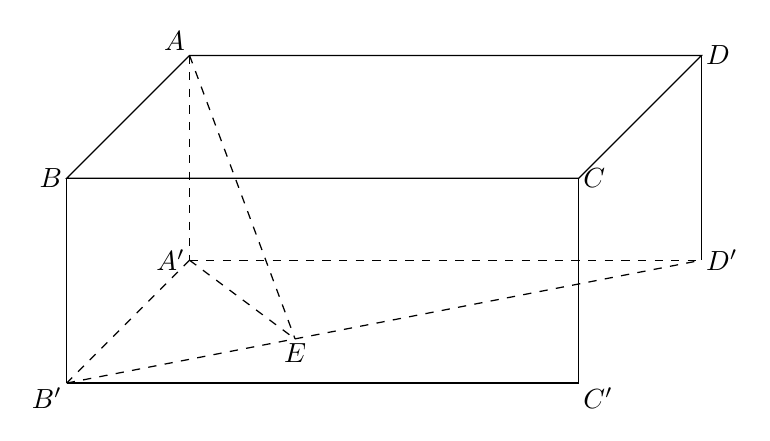
\begin{tikzpicture}[scale=1, line width=0.45pt,
  every node/.style={inner sep=1.5pt}]
  % 顶点（斜二测投影手算：宽 8 单位 -> 6.5cm 水平；深 6 单位 -> 2.2cm 左下 45 度；
  % 高 3.6 单位 -> 2.6cm 竖直）
  \coordinate (A)  at (2.40, 5.80);
  \coordinate (B)  at (0.84, 4.24);
  \coordinate (C)  at (7.34, 4.24);
  \coordinate (D)  at (8.90, 5.80);
  \coordinate (Ap) at (2.40, 3.20);
  \coordinate (Bp) at (0.84, 1.64);
  \coordinate (Cp) at (7.34, 1.64);
  \coordinate (Dp) at (8.90, 3.20);
  % E 为 B'D' 上一点，B'E:B'D' = 3.6:10
  \coordinate (E)  at (3.74, 2.20);
  % 可见棱
  \draw (A) -- (B) -- (C) -- (D) -- cycle;
  \draw (B) -- (Bp);
  \draw (C) -- (Cp);
  \draw (D) -- (Dp);
  \draw (Bp) -- (Cp);
  % 不可见棱（虚线）
  \draw[dashed] (A) -- (Ap);
  \draw[dashed] (Ap) -- (Bp);
  \draw[dashed] (Ap) -- (Dp);
  \draw[dashed] (Bp) -- (Dp);
  \draw[dashed] (A) -- (E);
  \draw[dashed] (Ap) -- (E);
  % 顶点标注
  \node[anchor=south east] at (A)  {$A$};
  \node[anchor=east]       at (B)  {$B$};
  \node[anchor=west]       at (C)  {$C$};
  \node[anchor=west]       at (D)  {$D$};
  \node[anchor=east]       at (Ap) {$A'$};
  \node[anchor=north east] at (Bp) {$B'$};
  \node[anchor=north west] at (Cp) {$C'$};
  \node[anchor=west]       at (Dp) {$D'$};
  \node[anchor=north]      at (E)  {$E$};
\end{tikzpicture}
\end{center}
\nopagebreak[4]
\Needspace{4\baselineskip}
\textbf{解析}
\nopagebreak[4]
\begin{center}% 1980 年全国卷（文科）第 7 题：长方体 ABCD-A'B'C'D'（AB=6、AD=8、AA'=3.6），底面对角线 B'D' 及 AE、A'E（E 为垂足）；左上、显示 A-A' 等被遮棱为虚线（按源卷布局）
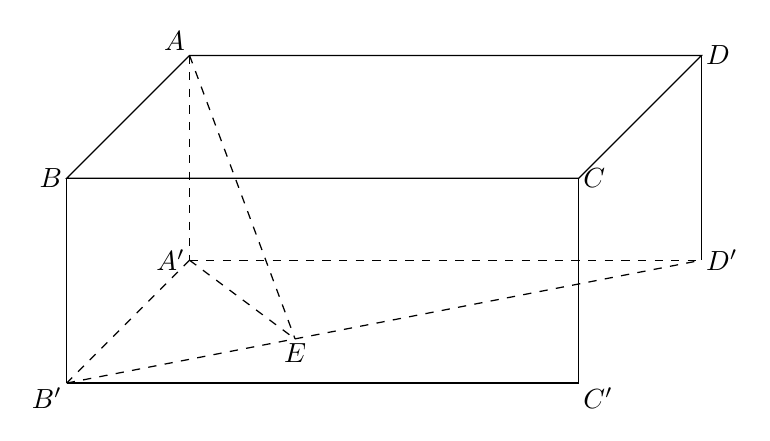
\begin{tikzpicture}[scale=1, line width=0.45pt,
  every node/.style={inner sep=1.5pt}]
  % 顶点（斜二测投影手算：宽 8 单位 -> 6.5cm 水平；深 6 单位 -> 2.2cm 左下 45 度；
  % 高 3.6 单位 -> 2.6cm 竖直）
  \coordinate (A)  at (2.40, 5.80);
  \coordinate (B)  at (0.84, 4.24);
  \coordinate (C)  at (7.34, 4.24);
  \coordinate (D)  at (8.90, 5.80);
  \coordinate (Ap) at (2.40, 3.20);
  \coordinate (Bp) at (0.84, 1.64);
  \coordinate (Cp) at (7.34, 1.64);
  \coordinate (Dp) at (8.90, 3.20);
  % E 为 B'D' 上一点，B'E:B'D' = 3.6:10
  \coordinate (E)  at (3.74, 2.20);
  % 可见棱
  \draw (A) -- (B) -- (C) -- (D) -- cycle;
  \draw (B) -- (Bp);
  \draw (C) -- (Cp);
  \draw (D) -- (Dp);
  \draw (Bp) -- (Cp);
  % 不可见棱（虚线）
  \draw[dashed] (A) -- (Ap);
  \draw[dashed] (Ap) -- (Bp);
  \draw[dashed] (Ap) -- (Dp);
  \draw[dashed] (Bp) -- (Dp);
  \draw[dashed] (A) -- (E);
  \draw[dashed] (Ap) -- (E);
  % 顶点标注
  \node[anchor=south east] at (A)  {$A$};
  \node[anchor=east]       at (B)  {$B$};
  \node[anchor=west]       at (C)  {$C$};
  \node[anchor=west]       at (D)  {$D$};
  \node[anchor=east]       at (Ap) {$A'$};
  \node[anchor=north east] at (Bp) {$B'$};
  \node[anchor=north west] at (Cp) {$C'$};
  \node[anchor=west]       at (Dp) {$D'$};
  \node[anchor=north]      at (E)  {$E$};
\end{tikzpicture}
\end{center}
\nopagebreak[4]
\Needspace{5\baselineskip}
长方体 $ABCD\text{-}A'B'C'D'$ 中 $ABCD$ 为上底面、$A'B'C'D'$ 为下底面，$AA'$、$BB'$、$CC'$、$DD'$ 为侧棱，且
\nopagebreak[4]
\[
A'B'=AB=6,\qquad A'D'=AD=8,\qquad AA'=3.6.
\]

\gksubpart{（1）}

\Needspace{5\baselineskip}
因 $AA'\perp$ 底面 $A'B'C'D'$，点 $A$ 在底面上的射影为 $A'$；点 $E$ 在底面内，其射影即自身，故直线 $AE$ 在底面上的射影为直线 $A'E$。又已知 $AE\perp B'D'$（垂足为 $E$），由三垂线定理
\nopagebreak[4]
\[
A'E\perp B'D'.
\]

（亦可不依赖三垂线定理：设 $E$ 为 $AE$ 与 $B'D'$ 的交点。把 $AE$、$A'E$ 分解为竖直分量与水平分量，$AE\perp B'D'$ 的两线段数量积为 $0$，其中竖直分量与 $B'D'$ 的数量积恒为 $0$，故水平分量 $A'E$ 与 $B'D'$ 的数量积也为 $0$，即 $A'E\perp B'D'$。）

\gksubpart{（2）}

\Needspace{5\baselineskip}
下底面 $A'B'C'D'$ 是边长为 $6$、$8$ 的矩形，在直角三角形 $A'B'D'$（直角在 $A'$）中
\nopagebreak[4]
\[
B'D'=\sqrt{6^2+8^2}=10.
\]
\Needspace{5\baselineskip}
$A'E$ 是斜边 $B'D'$ 上的高，由面积关系
\nopagebreak[4]
\[
A'E=\frac{A'B'\cdot A'D'}{B'D'}=\frac{6\times8}{10}=4.8.
\]
\Needspace{5\baselineskip}
又 $AA'\perp$ 底面，故 $AA'\perp A'E$，在直角三角形 $AEA'$（直角在 $A'$）中
\nopagebreak[4]
\[
AE=\sqrt{AA'^2+A'E^2}=\sqrt{3.6^2+4.8^2}=\sqrt{12.96+23.04}=\sqrt{36}=6.
\]

\Needspace{5\baselineskip}
复算（坐标法）：取 $A'(0,0,0)$、$B'(6,0,0)$、$D'(0,8,0)$、$A(0,0,3.6)$，则 $B'D'$ 上垂足
\nopagebreak[4]
\[
E=B'+\frac{3.6}{10}(D'-B')=(6,0,0)+0.36\,(-6,8,0)=(3.84,\ 2.88,\ 0).
\]
于是 $\overrightarrow{AE}=(3.84,2.88,-3.6)$，$\overrightarrow{A'E}=(3.84,2.88,0)$，$|\overrightarrow{A'E}|=\sqrt{3.84^2+2.88^2}=\sqrt{14.7456+8.2944}=\sqrt{23.04}=4.8$，$|\overrightarrow{AE}|=\sqrt{23.04+12.96}=\sqrt{36}=6$；且 $\overrightarrow{AE}\cdot\overrightarrow{B'D'}=(3.84,2.88,-3.6)\cdot(-6,8,0)=-23.04+23.04+0=0$、$\overrightarrow{A'E}\cdot\overrightarrow{B'D'}=-23.04+23.04+0=0$，两垂直关系同时成立，与 (1) 结论一致。

\gkanswer{答案（1）：见解析版}

\gkanswer{答案（2）：$AE=6$}

\end{answer}
\begin{answer}
\gksolhead{8}{}

\textbf{题目}：

\Needspace{5\baselineskip}
（1） 把参数方程
\nopagebreak[4]
\[
\begin{cases}
x=\sec t,\\
y=2\tan t
\end{cases}
\quad(t\ \text{为参数})
\]
化为直角坐标方程，并画出方程的曲线的略图；

（2） 当 $0\le t<\dfrac{\pi}{2}$ 及 $\pi\le t<\dfrac{3\pi}{2}$ 时，各得到曲线的哪一部分？

\Needspace{4\baselineskip}
\textbf{解析}

\gksubpart{（1）}

\Needspace{5\baselineskip}
由 $x=\sec t$、$y=2\tan t$ 得
\nopagebreak[4]
\[
x^2=\sec^2t,\qquad \frac{y^2}{4}=\tan^2t.
\]
\Needspace{5\baselineskip}
相减，利用恒等式 $\sec^2t-\tan^2t=1$：
\nopagebreak[4]
\[
x^2-\frac{y^2}{4}=1.
\]
\Needspace{5\baselineskip}
这是中心在原点、实轴在 $x$ 轴上的双曲线，$a=1$、$b=2$，顶点为 $(\pm1,0)$，渐近线为
\nopagebreak[4]
\[
\frac{y^2}{4}=x^2\ \Longrightarrow\ y=\pm2x.
\]
又因 $|x|=|\sec t|\ge1$，曲线只在 $|x|\ge1$ 处有实点。

略图：在坐标平面内画出 $y=\pm2x$ 两条虚线渐近线，再描出双曲线的左、右两支，标出顶点 $(\pm1,0)$。

\gksubpart{（2）}

\Needspace{5\baselineskip}
当 $0\le t<\dfrac{\pi}{2}$ 时：
\nopagebreak[4]
\[
x=\sec t\ge1\ (\text{由 }1\text{ 增到 }+\infty),\qquad y=2\tan t\ge0\ (\text{由 }0\text{ 增到 }+\infty),
\]
即 $x\ge1$、$y\ge0$，得到\textbf{右支在 $x$ 轴上方的部分}（含顶点 $(1,0)$）。

\Needspace{5\baselineskip}
当 $\pi\le t<\dfrac{3\pi}{2}$ 时，$t$ 在第三象限：
\nopagebreak[4]
\[
x=\sec t\le-1\ (\text{由 }-1\text{ 减到 }-\infty),\qquad y=2\tan t\ge0\ (\text{由 }0\text{ 增到 }+\infty),
\]
即 $x\le-1$、$y\ge0$，得到\textbf{左支在 $x$ 轴上方的部分}（含顶点 $(-1,0)$）。

复算：$t=\dfrac{\pi}{4}$ 给 $\left(\sqrt2,\ 2\right)$，$x^2-\dfrac{y^2}{4}=2-1=1$ ，且 $x>1$、$y>0$；$t=\dfrac{5\pi}{4}$ 给 $\left(-\sqrt2,\ 2\right)$，$x^2-\dfrac{y^2}{4}=2-1=1$ ，且 $x<-1$、$y>0$；端点 $t=\pi$ 给 $(-1,0)$，确在左支顶点。可知两段分别对应右支上半、左支上半。

\gkanswer{答案（1）：$x^2-\dfrac{y^2}{4}=1$（双曲线，中心在原点，实轴在 $x$ 轴，$a=1$、$b=2$，渐近线 $y=\pm2x$）}

\gkanswer{答案（2）：当 $0\le t<\dfrac{\pi}{2}$ 时得到双曲线右支在 $x$ 轴上方的部分（含顶点 $(1,0)$）；当 $\pi\le t<\dfrac{3\pi}{2}$ 时得到左支在 $x$ 轴上方的部分（含顶点 $(-1,0)$）}

\end{answer}